\documentclass{article}
\usepackage[utf8]{inputenc}
\usepackage[english]{babel}
\usepackage[]{amsthm}
\usepackage[]{amssymb}
\usepackage[]{amsmath}
\usepackage{graphicx}
\usepackage{listings}
\lstset{language=Matlab}

\title{SP21 COMPSCI 513 - Homework 4}
\author{Zijie Zhang}
\date\today

\begin{document}
\maketitle
\section*{Q1}
    \begin{itemize}
        \item[(a)]
        $(\lambda, v)$ is an eigenpair of $B$ means
        $$Bv = \lambda v$$
        We know that $B$ is invertible, then $B^{-1}$ exists. It gives
        $$B^{-1}Bv = B^{-1}\lambda v = \lambda B^{-1}v = v$$
        $$B^{-1}v =\lambda^{-1} v$$
        This means $(1/\lambda, v)$ is an eigenpair of $B^{-1}$.\\
        The entire proof is equivalent and reversible.
        \item[(b)]
        By definition, $$\left\Vert A^{-1} \right\Vert_2 = \sqrt{\rho((AA')^{-1})}$$
        i.e. $$\left\Vert A^{-1} \right\Vert_2 = \sqrt{\max{\{|\lambda|:\lambda\in\sigma((AA')^{-1}) \}} } $$
        By the statement in (a)
        $$\left\Vert A^{-1} \right\Vert_2 = \sqrt{\max{\{|1/\lambda|:\lambda\in\sigma(AA') \}} } = 1/\sqrt{\min{\{|\lambda|:\lambda\in\sigma(AA') \}} } $$
        $\left\Vert A^{-1} \right\Vert_2$ is the absolute value of reciprocal of the singular value of $A$ with the smallest absolute value.
    \end{itemize}
\section*{Q2}
    \begin{itemize}
        \item[(a)]
        $(\lambda, v)$ is an eigenpair of $A'A$ if and only if $(\sqrt{\lambda}, v)$ or $(-\sqrt{\lambda}, v)$ is an eigenpair of $A$.\\
            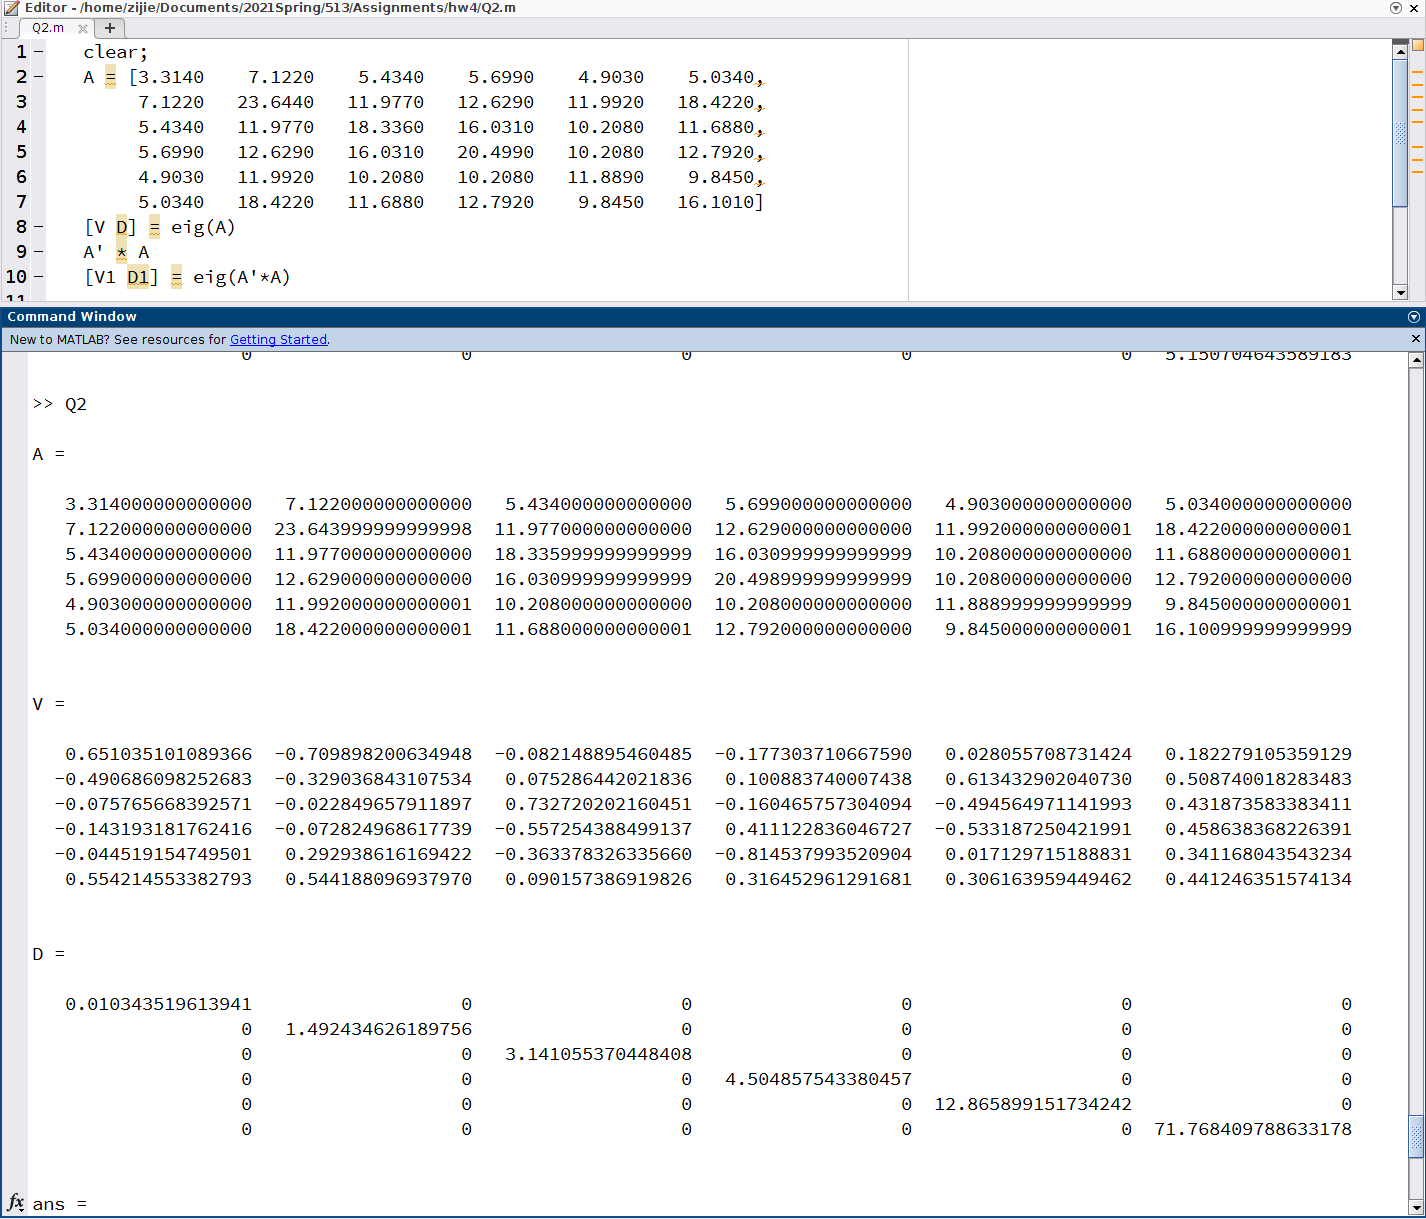
\includegraphics[width=6cm]{a1.png}
            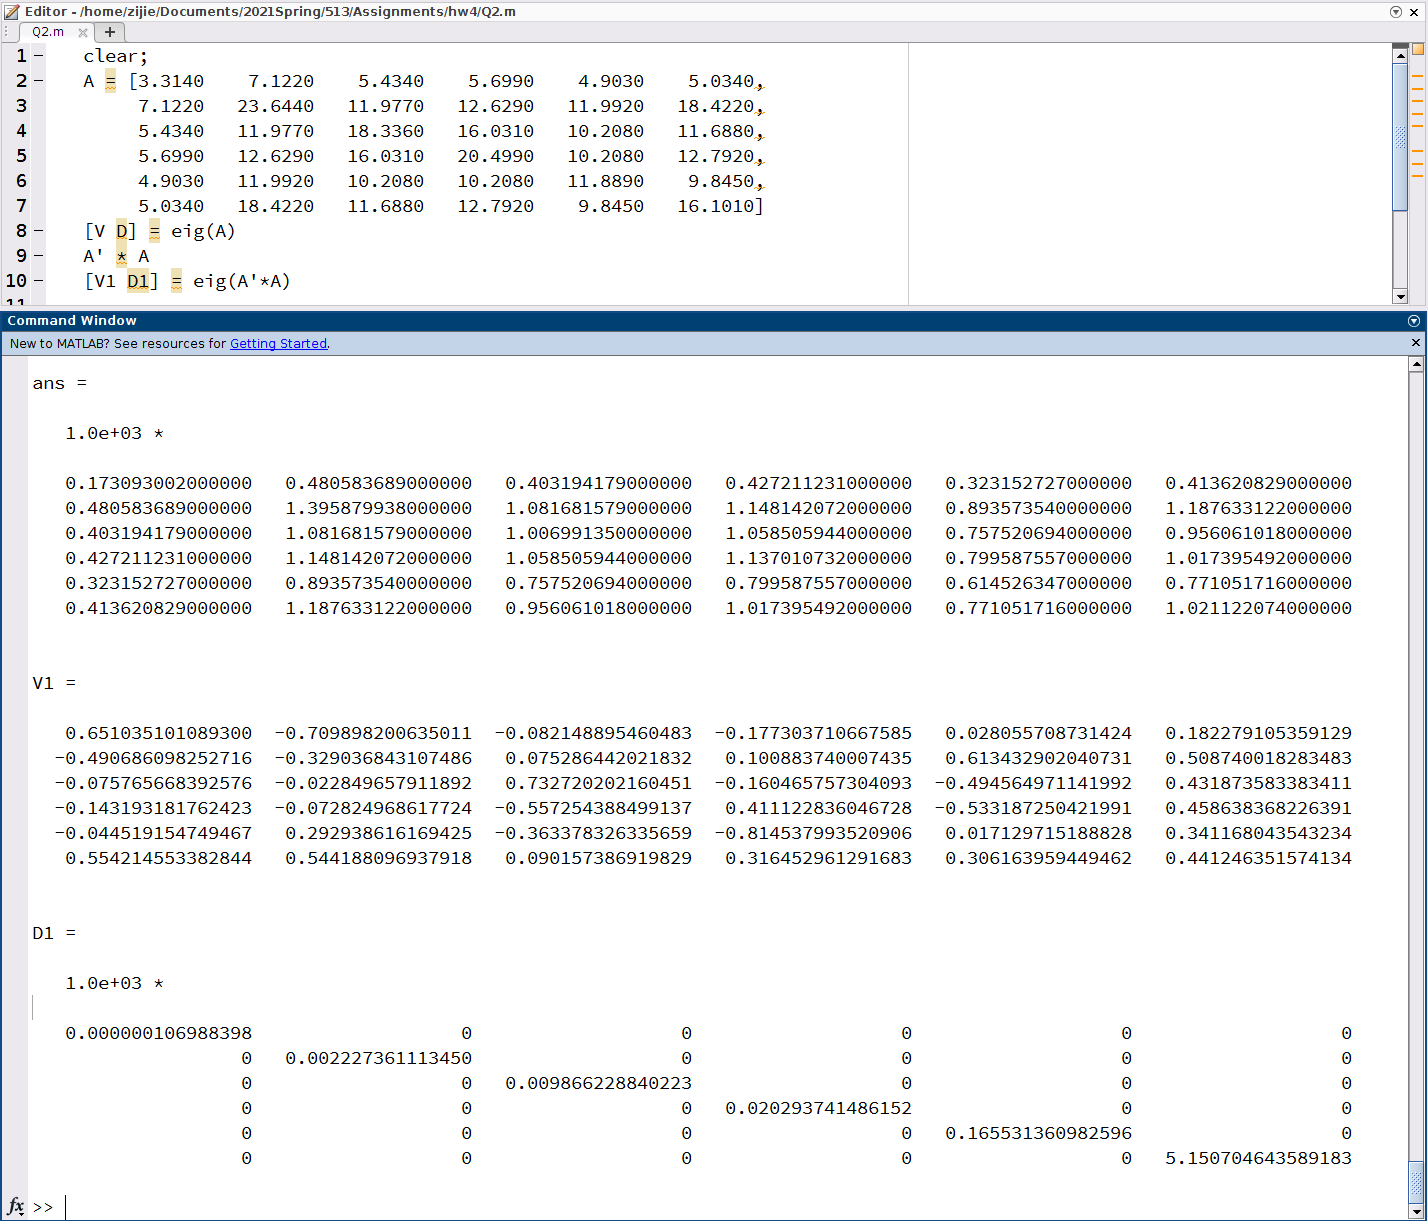
\includegraphics[width=6cm]{a2.png}
        \item[(b)]
        If $(\lambda, v)$ is an eigenpair of $A'A$, then we have
        $$A'Av = \lambda v$$
        We know that $A$ is symmetric, $A'A = A^2$, which means, we can find the square root of $A^2$. Obviously, every eigenvalue is unique by the special property. Then, it gives
        $$Av = \sqrt{\lambda}v \quad\text{or}\quad Av = -\sqrt{\lambda}v$$
        If $(\sqrt{\lambda}, v)$ or $(-\sqrt{\lambda}, v)$ is an eigenpair of $A$. Condsider $(\sqrt{\lambda}, v)$ is an eigenpair of $A$, it gives
        $$Av = \sqrt{\lambda}v, A'v = \sqrt{\lambda}v$$
        $$A'Av = \lambda v$$
        \item[(c)]
        Check with MATLAB.\\
        True.\\
        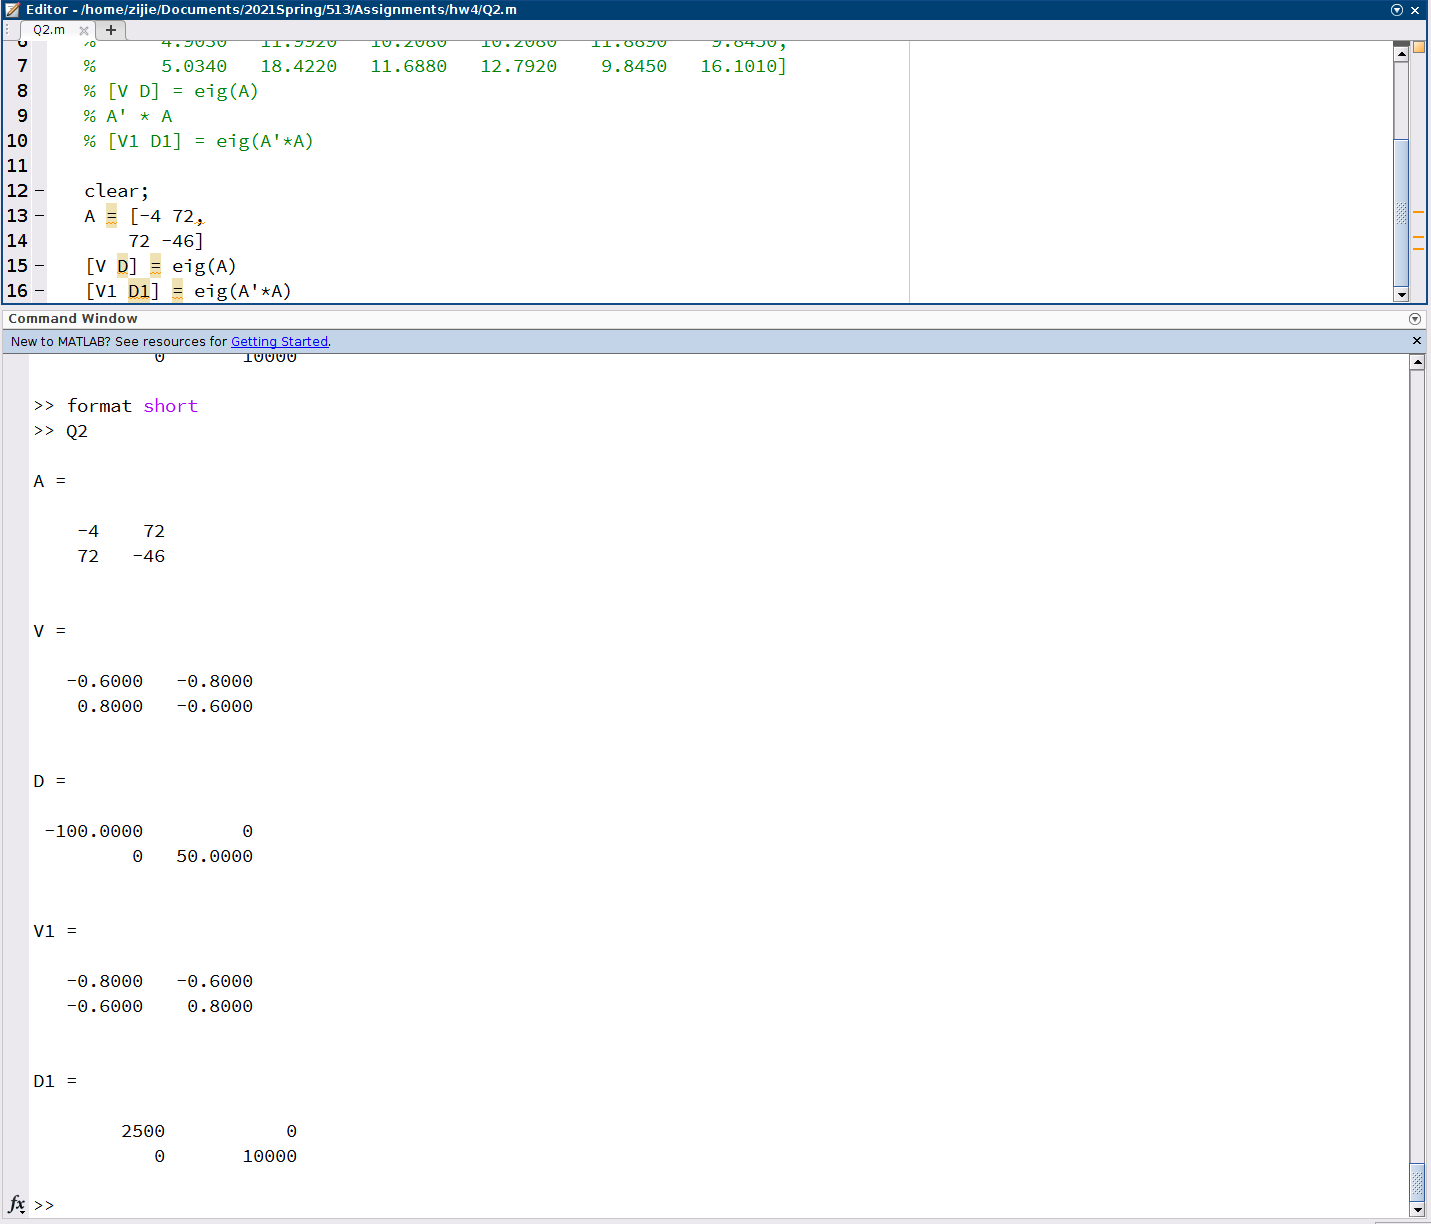
\includegraphics[width=8cm]{c.png}
        \item[(d)]
        $$A = \begin{bmatrix}
            1 &3\\
            3 &-1\\
        \end{bmatrix}$$
        \begin{lstlisting}
            V = [0.5847   -0.8112
                -0.8112   -0.5847]
            D = [-3.1623        0
                0          3.1623]
        \end{lstlisting}
        $$A'A = \begin{bmatrix}
            10 &0\\
            0  &10\\
        \end{bmatrix}$$
        Obviously, this theorem does not hold.
    \end{itemize}
\end{document}